% 1977 年广西卷（理科）第 3 题：四边形 ABCD，E、F 为对角线 AC、BD 的中点，M、N 为 AB、CD 的中点，
% 虚线四边形 EMFN 为平行四边形，MN、EF 是其对角线（按源卷第 2 页布局）
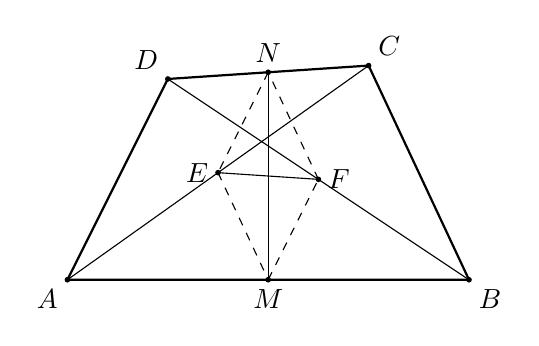
\begin{tikzpicture}[scale=0.85]
  \coordinate (A) at (0,0);
  \coordinate (B) at (6,0);
  \coordinate (D) at (1.5,3);
  \coordinate (C) at (4.5,3.2);
  \coordinate (M) at (3,0);
  \coordinate (N) at (3,3.1);
  \coordinate (E) at (2.25,1.6);
  \coordinate (F) at (3.75,1.5);
  \draw[thick] (A)--(B)--(C)--(D)--cycle;
  \draw[thin] (A)--(C);
  \draw[thin] (B)--(D);
  \draw (E)--(F);
  \draw (M)--(N);
  \draw[dashed] (E)--(M) (M)--(F) (F)--(N) (N)--(E);
  \fill (A) circle (1.2pt) node[below left] {$A$};
  \fill (B) circle (1.2pt) node[below right] {$B$};
  \fill (C) circle (1.2pt) node[above right] {$C$};
  \fill (D) circle (1.2pt) node[above left] {$D$};
  \fill (M) circle (1.2pt) node[below] {$M$};
  \fill (N) circle (1.2pt) node[above] {$N$};
  \fill (E) circle (1.2pt) node[left] {$E$};
  \fill (F) circle (1.2pt) node[right] {$F$};
\end{tikzpicture}
